\chapter{Kleurgebaseerde similariteitsmaten}

In dit hoofdstuk construeren we enkele similariteitsmaten die beelden 
vergelijken op basis van de kleuren die er in voorkomen. We identificeren de beelden
in dit geval dus met vaagverzamelingen in een universum dat bestaat uit kleuren 
in plaats van beeldpunten. Vermits kleur \'e\'en  van de meest gebruikte kenmerken is bij CBIR 
\cite{rui:image_retr, schettini:survey_of_methods_for_colour_image_indexing_and_retrieval}, mogen we 
verwachten dat die \emph{kleurgebaseerde} aanpak effici\"ente 
similariteitsmaten zal opleveren. 

\section{Histogrammen}

Een \emph{histogram} van een kleurbeeld is een voorstelling van de frequentieverdeling 
van de verschillende kleuren. De waarde van het histogram voor een kleurbeeld 
$A$ in de kleur $c \in C$ is dus gelijk aan het totaal aantal pixels in het beeld met 
kleur $c$. Om de complexiteit te beperken wordt er in de praktijk gebruik gemaakt
van kleurkwantisatie. Het universum der kleuren $C$ wordt dus beperkt tot $C' \subset C$. 
%Het histogram wordt dus berekend voor verzamelingen van
%kleuren in plaats van individuele kleuren. 
De waarde van het histogram voor een beeld $A$ in de kleur $c \in C'$ is dan gelijk aan 
het totaal aantal pixels in $A$ die tot bin $bin(c)$ behoren. Met andere woorden: het histogram 
geeft de frequentieverdeling weer van de kleuren uit $C'$ in de gekwantiseerde versie van 
$A$. We noteren de waarde in $c$ van het histogram van een beeld $A$ met $h_A(c)$: 
\begin{displaymath}
h_A(c) = \sum_{p \in P} \delta (bin(c) - bin(A(p))) 
\end{displaymath} 
waarbij $\delta$ de Diracfuntie is ($\delta (0)=1$ en $\delta (x)=0$ voor alle 
$x \in \mathbb{Z} \setminus \{0\}$) en $P$ het universum der beeldpunten 
voorstelt. De functie $bin$ is uiteraard de $C - \{1,2,\ldots,N\}$ afbeelding 
uit \ref{sectie:kleurkwantisatie}, die met 
elke kleur het nummer van \'e\'en van de $N$ bins associeert. 


\subsection{Pseudo-vage histogrammen}

Door de waarden van een histogram te normaliseren, kunnen we het omzetten naar 
een vaagverzameling in het universum der kleuren $C'$ 
\cite{debaets:similariteitsmaten_voor_kleurbeelden, vanderweken:similariteitsmaten, vertan:embedding_fuzzy_logic_in_cbir}. 
Dat houdt in dat we elke 
waarde van het histogram delen door het maximaal aantal pixels met dezelfde 
kleur. We hebben dus de volgende uitdrukking voor de lidmaatschapsgraad van de 
kleur $c \in C$ in de vaagverzameling $H_A$ geassocieerd met het histogram 
van beeld $A$: 
\begin{displaymath}
H_A(c) = \frac{\displaystyle h_A(c)}{\displaystyle \max_{c \in C'}(h_A(c))}
\end{displaymath}
Een dergelijke vaagverzameling noemen we een \emph{pseudo-vaag histogram}. 
De kleur die het meest voorkomt heeft daarbij lidmaatschapsgraad $1$. Alle 
andere kleuren hebben kleinere lidmaatschapsgraden. 

We beschouwen de zes uniforme en de eerste twee niet-uniforme (focale kleuren en SCT) 
kwantisatietechnieken uit \ref{sectie:kleurkwantisatie}. Figuur~\ref{fig:histogrammen_eerste_vb} bevat
de pseudo-vage histogrammen die we zo bekomen voor het ``geel bootje'' voorbeeld
uit onze testcollectie. In figuur~\ref{fig:alle_histn_geel_bootje} worden de pseudo-vage histogrammen
getoond van alle beelden uit de testcollectie die relevant zijn ten opzichte van dat voorbeeld.

\begin{figure}[!bp]
\vspace{2pt}
\centering
\begin{tabular}{c}
\subfigure[] {
\begin{minipage}[c]{0.3\textwidth}
\begin{center}
\includegraphics[height=2.7cm, width=\textwidth]{images/hist_hsv_obj3__0.eps}
\end{center}
\vspace{1pt}
\end{minipage}
}
\subfigure[] {
\begin{minipage}[c]{0.3\textwidth}
\begin{center}
\includegraphics[height=2.7cm, width=\textwidth]{images/hist_irb_obj3__0.eps}
\end{center}
\vspace{1pt}
\end{minipage}
}
\subfigure[] {
\begin{minipage}[c]{0.3\textwidth}
\begin{center}
\includegraphics[height=2.7cm, width=\textwidth]{images/hist_i1i2i3_obj3__0.eps}
\end{center}
\vspace{1pt}
\end{minipage}
}\\
\subfigure[] {
\begin{minipage}[c]{0.3\textwidth}
\begin{center}
\includegraphics[height=2.7cm, width=\textwidth]{images/hist_xyz_obj3__0.eps}
\end{center}
\vspace{1pt}
\end{minipage}
}
\subfigure[] {
\begin{minipage}[c]{0.3\textwidth}
\begin{center}
\includegraphics[height=2.7cm, width=\textwidth]{images/hist_yxy_obj3__0.eps}
\end{center}
\vspace{1pt}
\end{minipage}
}
\subfigure[] {
\begin{minipage}[c]{0.3\textwidth}
\begin{center}
\includegraphics[height=2.7cm, width=\textwidth]{images/hist_lab_obj3__0.eps}
\end{center}
\vspace{1pt}
\end{minipage}
}\\
\subfigure[] {
\begin{minipage}[c]{0.1\textwidth}
\begin{center}
\includegraphics[height=2.7cm, width=\textwidth]{images/hist_focal_obj3__0.eps}
\end{center}
\vspace{1pt}
\end{minipage}
}
\subfigure[] {
\begin{minipage}[c]{0.3\textwidth}
\begin{center}
\includegraphics[height=2.7cm, width=\textwidth]{images/hist_sct_obj3__0.eps}
\end{center}
\vspace{1pt}
\end{minipage}
}
\subfigure[] {
\begin{minipage}[c]{0.5\textwidth}
\begin{center}
\includegraphics[height=2.7cm, width=\textwidth]{images/hist_fuzzy_obj3__0.eps}
\end{center}
\vspace{1pt}
\end{minipage}
\label{fig:vaaghistogram_eerste_vb}
}
\end{tabular}
\caption{\label{fig:histogrammen_eerste_vb}De verschillende histogrammen voor het ``geel bootje'' 
voorbeeld (HSV (a), Irb (b), I1I2I3 (c), XYZ (d), Yxy (e) en L*a*b* (f), focale kleuren (g), SCT (h) 
en het vaaghistogram voor $\lambda = 5$ (i)).}
\end{figure}

\begin{figure}[bp]
\vspace{5pt}
\centering
%\subfigure[] {
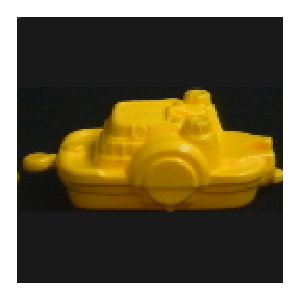
\includegraphics[width=2.5cm]{coil/beeld-12.eps}
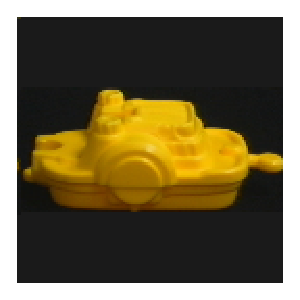
\includegraphics[width=2.5cm]{coil/beeld-13.eps}
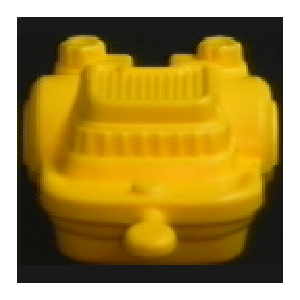
\includegraphics[width=2.5cm]{coil/beeld-14.eps}
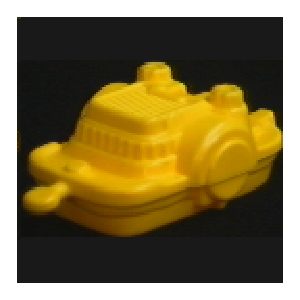
\includegraphics[width=2.5cm]{coil/beeld-15.eps}
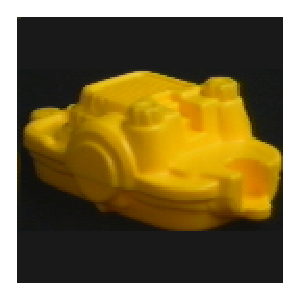
\includegraphics[width=2.5cm]{coil/beeld-16.eps}
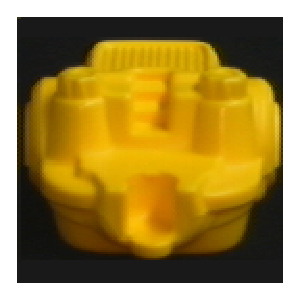
\includegraphics[width=2.5cm]{coil/beeld-17.eps}\\[4pt]
%}
\vspace{3pt}
\subfigure[] {
\includegraphics[width=2.5cm]{images/hist_hsv_obj3__0.eps}
\includegraphics[width=2.5cm]{images/hist_hsv_obj3__45.eps}
\includegraphics[width=2.5cm]{images/hist_hsv_obj3__90.eps}
\includegraphics[width=2.5cm]{images/hist_hsv_obj3__180.eps}
\includegraphics[width=2.5cm]{images/hist_hsv_obj3__270.eps}
\includegraphics[width=2.5cm]{images/hist_hsv_obj3__315.eps}
}
\subfigure[] {
\includegraphics[width=2.5cm]{images/hist_irb_obj3__0.eps}
\includegraphics[width=2.5cm]{images/hist_irb_obj3__45.eps}
\includegraphics[width=2.5cm]{images/hist_irb_obj3__90.eps}
\includegraphics[width=2.5cm]{images/hist_irb_obj3__180.eps}
\includegraphics[width=2.5cm]{images/hist_irb_obj3__270.eps}
\includegraphics[width=2.5cm]{images/hist_irb_obj3__315.eps}
}
\subfigure[] {
\includegraphics[width=2.5cm]{images/hist_i1i2i3_obj3__0.eps}
\includegraphics[width=2.5cm]{images/hist_i1i2i3_obj3__45.eps}
\includegraphics[width=2.5cm]{images/hist_i1i2i3_obj3__90.eps}
\includegraphics[width=2.5cm]{images/hist_i1i2i3_obj3__180.eps}
\includegraphics[width=2.5cm]{images/hist_i1i2i3_obj3__270.eps}
\includegraphics[width=2.5cm]{images/hist_i1i2i3_obj3__315.eps}
}
\subfigure[] {
\includegraphics[width=2.5cm]{images/hist_xyz_obj3__0.eps}
\includegraphics[width=2.5cm]{images/hist_xyz_obj3__45.eps}
\includegraphics[width=2.5cm]{images/hist_xyz_obj3__90.eps}
\includegraphics[width=2.5cm]{images/hist_xyz_obj3__180.eps}
\includegraphics[width=2.5cm]{images/hist_xyz_obj3__270.eps}
\includegraphics[width=2.5cm]{images/hist_xyz_obj3__315.eps}
}
\subfigure[] {
\includegraphics[width=2.5cm]{images/hist_yxy_obj3__0.eps}
\includegraphics[width=2.5cm]{images/hist_yxy_obj3__45.eps}
\includegraphics[width=2.5cm]{images/hist_yxy_obj3__90.eps}
\includegraphics[width=2.5cm]{images/hist_yxy_obj3__180.eps}
\includegraphics[width=2.5cm]{images/hist_yxy_obj3__270.eps}
\includegraphics[width=2.5cm]{images/hist_yxy_obj3__315.eps}
}
\subfigure[] {
\includegraphics[width=2.5cm]{images/hist_lab_obj3__0.eps}
\includegraphics[width=2.5cm]{images/hist_lab_obj3__45.eps}
\includegraphics[width=2.5cm]{images/hist_lab_obj3__90.eps}
\includegraphics[width=2.5cm]{images/hist_lab_obj3__180.eps}
\includegraphics[width=2.5cm]{images/hist_lab_obj3__270.eps}
\includegraphics[width=2.5cm]{images/hist_lab_obj3__315.eps}
}
\subfigure[] {
\includegraphics[width=1cm,height=2.5cm,angle=-90]{images/hist_focal_obj3__0.eps}
\includegraphics[width=1cm,height=2.5cm,angle=-90]{images/hist_focal_obj3__45.eps}
\includegraphics[width=1cm,height=2.5cm,angle=-90]{images/hist_focal_obj3__90.eps}
\includegraphics[width=1cm,height=2.5cm,angle=-90]{images/hist_focal_obj3__180.eps}
\includegraphics[width=1cm,height=2.5cm,angle=-90]{images/hist_focal_obj3__270.eps}
\includegraphics[width=1cm,height=2.5cm,angle=-90]{images/hist_focal_obj3__315.eps}
}
\subfigure[] {
\includegraphics[width=2.5cm]{images/hist_sct_obj3__0.eps}
\includegraphics[width=2.5cm]{images/hist_sct_obj3__45.eps}
\includegraphics[width=2.5cm]{images/hist_sct_obj3__90.eps}
\includegraphics[width=2.5cm]{images/hist_sct_obj3__180.eps}
\includegraphics[width=2.5cm]{images/hist_sct_obj3__270.eps}
\includegraphics[width=2.5cm]{images/hist_sct_obj3__315.eps}
}
\caption{\label{fig:alle_histn_geel_bootje}De verschillende pseudo-vage histogrammen voor de beelden 
van het geel bootje (HSV (a), Irb (b), I1I2I3 (c), XYZ (d), Yxy (e) en L*a*b* (f), focale kleuren (g) en SCT (h)).}
\end{figure}

\begin{figure}[bp]
\vspace{5pt}
\centering
\includegraphics[height=2cm]{coil/beeld-12.eps}
\includegraphics[height=2cm]{images/hist_fuzzy_obj3__0.eps}\hspace{1cm}
\includegraphics[height=2cm]{coil/beeld-13.eps}
\includegraphics[height=2cm]{images/hist_fuzzy_obj3__45.eps}\\[5pt]
\includegraphics[height=2cm]{coil/beeld-14.eps}
\includegraphics[height=2cm]{images/hist_fuzzy_obj3__90.eps}\hspace{1cm}
\includegraphics[height=2cm]{coil/beeld-15.eps}
\includegraphics[height=2cm]{images/hist_fuzzy_obj3__180.eps}\\[5pt]
\includegraphics[height=2cm]{coil/beeld-12.eps}
\includegraphics[height=2cm]{images/hist_fuzzy_obj3__270.eps}\hspace{1cm}
\includegraphics[height=2cm]{coil/beeld-12.eps}
\includegraphics[height=2cm]{images/hist_fuzzy_obj3__315.eps}
\vspace{5pt}
\caption{\label{fig:alle_vaaghistn_geel_bootje}De verschillende vaaghistogrammen voor de beelden 
van het geel bootje.}
\end{figure}

%Voor een RGB-beeld gebruikt men typisch 8 bits per kleurcomponent. Dit geeft een totaal van
%24 bits per kleur, zodat men dus $2^{24}=2^4 \cdot 2^{20}=16 \cdot 2^{20} \approx 16 \cdot 10^6$
%kleuren kan voorstellen. Een genormaliseerd histogram bestaat dan dus uit 16 miljoen waarden.
%Similariteitsmaten op basis van dergelijke histogrammen zouden dus veel te veel rekentijd vragen.

\subsection{Vaaghistogrammen}

Naast de bovenstaande vage interpretatie van het klassieke kleurhistogram, 
beschouwen we ook nog een gelijkaardige kleurbeschrijving die we op een 
``volledig vage'' manier opbouwen. Bij dat \emph{vaaghistogram} maken we 
gebruik van het L*a*b* kleurmodel en beschouwen we een 
vaagverzameling voor elke kleur. Stel dat $lab$ de kleuren uit $C$ afbeeldt op de
corresponderende niet-genormaliseerde L*a*b*-co\"ordinaten. De lidmaatschapsgraad van een 
kleur $c' \in C$ in de vaagverzameling $\widetilde{C}_c$, die correspondeert met kleur $c \in C$, 
defini\"eren we dan als volgt \cite{vertan:fuzzy_histograms}:
\begin{displaymath}
\widetilde{C}_c(c') =
\begin{cases}
1 & \textrm{als } d'_{c,c'} = \frac{d \left( lab(c), lab(c') \right)}{2.3} \leq 1 \\ 
\exp \frac{- \left( d'_{c,c'} - 1 \right)^2}{2 \cdot \lambda^2} & \textrm{anders}
\end{cases}
\end{displaymath} 
met $d$ de Euclidische afstand en $\lambda$ een vrij te kiezen parameter. In 
het geval van (niet-ge\-nor\-ma\-li\-seer\-de) L*a*b* komt de afstand $2.3$ namelijk 
overeen met de zogenaamde 
\emph{just noticeable difference} (JND) \cite{sharma:digital_color_imaging}. 
Kleuren waarvan de onderlinge afstand kleiner dan of gelijk aan die JND is, 
kunnen door de mens niet onderscheiden worden.

Het eigenlijk vaaghistogram $\widetilde{H}_A$, voor een kleurbeeld $A$, defini\"eren we 
dan als de unie van alle kleuren die voorkomen in $A$: 
\begin{displaymath} 
\widetilde{H}_A = \displaystyle\bigcup_{c \in C_A} \widetilde{C}_c
%\begin{array}{lrcl}
%Vh_A: 	& C_A 	& \to 		& [0,1] \\[5pt]
%		& c					& \mapsto	& \displaystyle\bigcup_{c \in C_A} VC_c,
%\quad\forall c \in C_A
%\end{array}
\end{displaymath}
waarbij de verzameling $C_A \subseteq C$ bestaat uit de in $A$ voorkomende kleuren. Alle 
kleuren die (niet te onderscheiden zijn van kleuren die) voorkomen in het beeld 
hebben dus lidmaatschapsgraad $1$. De overige kleuren hebben kleinere 
lidmaatschapsgraden. 

Ook bij de vaaghistogrammen moeten we in de praktijk het kleurenuniversum $C$ 
kwantiseren om zo de complexiteit beperkt te houden. Vermits elke bin die een kleur
bevat die voorkomt dan lidmaatschapsgraad $1$ krijgt, mogen we evenwel niet te
ruw kwantiseren. Anders zou het discriminerend vermogen immers te laag worden. In deze
scriptie gebruiken we uniforme kwantisatie (in het L*a*b*-model) met $N_1=N_2=N_3=10$.
We reduceren $C$ dus tot 1000 kleuren. Voor het ``geel bootje'' voorbeeld uit de testcollectie
leidt dat tot het vaaghistogram uit figuur~\ref{fig:vaaghistogram_eerste_vb}. De vaaghistogrammen 
van alle beelden
uit de testcollectie die relevant zijn ten opzichte van dat voorbeeld, kunnen met
elkaar vergeleken worden in figuur~\ref{fig:alle_vaaghistn_geel_bootje}.

\subsection{Experimentele observaties}
\label{sectie:histogrammen_experimentele_observaties}

We vergelijken in deze sectie enkele similariteitsmaten die gebaseerd zijn op de bovenstaande
histogrammen. Voor de parameter $\lambda$ van het vaaghistogram gebruiken we daarbij
de waarde $5$.

Figuur~\ref{fig:histgeb_gggrs_en_cputimes} toont de bekomen meetresultaten. 
De corresponderende minimale en gemiddelde GGGR-waarden voor elk van de
vaagsimilariteitsmaten, worden weergegeven in 
tabel~\ref{tab:stat_gegevens_pseudo-vaag_histogram_maten}. Het Irb-histogram
en het XYZ-histogram geven, in combinatie met $M_{I3}$, de laagste GGGR-waarde. Hoewel die
waarde bij het Irb-histogram een fractie hoger is, merken we bij het vergelijken van 
figuur~\ref{fig:results_irb_histgeb} en figuur~\ref{fig:results_xyz_histgeb} dat het 
XYZ-histogram toch iets minder goede resultaten geeft. 

Uit de meetresultaten blijkt dat $M_5$, $M_{5c}$, $M_{11}$ en $M_{11c}$ in deze context
beduidend slechter presteren dan de overige vaagsimilariteitsmaten. Dat is niet
verwonderlijk, vermits die maten de enige zijn die de corresponderende bins van de histogrammen 
niet rechstreeks met elkaar vergelijken. Beschouw bijvoorbeeld een beeld $A$ dat enkel bestaat
uit rode beeldpunten en een beeld $B$ dat volledig groen is. In beide beelden komen alle
pixels in dezelfde bin terecht. Ze geven dus aanleiding tot pseudo-vage histogrammen $H_A$ en $H_B$  
die \'e\'en enkele piek bevatten, of tot vaaghistogrammen $\widetilde{H}_A$ en $\widetilde{H}_B$ 
waarbij er ook nog een aantal ``naburige'' bins een waarde hebben die verschilt van nul 
(zie figuur~\ref{fig:histogrammen_rood_en_groen}). 
\afterpage{\begin{figure}[bp]
\centering
\includegraphics[width=\textwidth]{/home/klbostee/Workspace/Thesis/plots/histgeb1_gggrs_en_cputimes_filled.eps} 
\includegraphics[width=\textwidth]{/home/klbostee/Workspace/Thesis/plots/histgeb2_gggrs_en_cputimes_filled.eps}
\includegraphics[width=\textwidth]{/home/klbostee/Workspace/Thesis/plots/histgeb3_gggrs_en_cputimes_filled.eps}
\vspace{1pt}
\caption{\label{fig:histgeb_gggrs_en_cputimes}De GGGR-waarde en de gebruikte rekentijd in ms voor elk 
van de similariteitsmaten op basis van histrogrammen.}
\end{figure}
%
\begin{figure}[bp]
\vspace{5pt}
\centering
\begin{tabular}{m{11cm} | m{3cm} |}
\textbf{Eerste tien resultaten:} & \textbf{GGR:} \\
\vspace{4pt}
\includegraphics[width=1cm]{coil/beeld-12.eps}
\includegraphics[width=1cm]{coil/beeld-13.eps}
\includegraphics[width=1cm]{coil/beeld-15.eps}
\includegraphics[width=1cm]{coil/beeld-16.eps}
\includegraphics[width=1cm]{coil/beeld-17.eps}
\includegraphics[width=1cm]{coil/beeld-14.eps}
\includegraphics[width=1cm]{coil/beeld-44.eps}
\includegraphics[width=1cm]{coil/beeld-47.eps}
\includegraphics[width=1cm]{coil/beeld-5.eps}
\includegraphics[width=1cm]{coil/beeld-2.eps}
& {\scriptsize 0.0}
\\
\includegraphics[width=1cm]{coil/beeld-6.eps}
\includegraphics[width=1cm]{coil/beeld-7.eps}
\includegraphics[width=1cm]{coil/beeld-8.eps}
\includegraphics[width=1cm]{coil/beeld-9.eps}
\includegraphics[width=1cm]{coil/beeld-11.eps}
\includegraphics[width=1cm]{coil/beeld-10.eps}
\includegraphics[width=1cm]{coil/beeld-65.eps}
\includegraphics[width=1cm]{coil/beeld-41.eps}
\includegraphics[width=1cm]{coil/beeld-64.eps}
\includegraphics[width=1cm]{coil/beeld-36.eps}
& {\scriptsize 0.0}
\\
\includegraphics[width=1cm]{coil/beeld-18.eps}
\includegraphics[width=1cm]{coil/beeld-19.eps}
\includegraphics[width=1cm]{coil/beeld-21.eps}
\includegraphics[width=1cm]{coil/beeld-22.eps}
\includegraphics[width=1cm]{coil/beeld-20.eps}
\includegraphics[width=1cm]{coil/beeld-23.eps}
\includegraphics[width=1cm]{coil/beeld-32.eps}
\includegraphics[width=1cm]{coil/beeld-36.eps}
\includegraphics[width=1cm]{coil/beeld-33.eps}
\includegraphics[width=1cm]{coil/beeld-39.eps}
& {\scriptsize 0.0}
\\
\includegraphics[width=1cm]{coil/beeld-24.eps}
\includegraphics[width=1cm]{coil/beeld-25.eps}
\includegraphics[width=1cm]{coil/beeld-28.eps}
\includegraphics[width=1cm]{coil/beeld-27.eps}
\includegraphics[width=1cm]{coil/beeld-26.eps}
\includegraphics[width=1cm]{coil/beeld-29.eps}
\includegraphics[width=1cm]{coil/beeld-39.eps}
\includegraphics[width=1cm]{coil/beeld-38.eps}
\includegraphics[width=1cm]{coil/beeld-7.eps}
\includegraphics[width=1cm]{coil/beeld-6.eps}
& {\scriptsize 0.0}
\\
\includegraphics[width=1cm]{coil/beeld-30.eps}
\includegraphics[width=1cm]{coil/beeld-32.eps}
\includegraphics[width=1cm]{coil/beeld-31.eps}
\includegraphics[width=1cm]{coil/beeld-33.eps}
\includegraphics[width=1cm]{coil/beeld-34.eps}
\includegraphics[width=1cm]{coil/beeld-35.eps}
\includegraphics[width=1cm]{coil/beeld-60.eps}
\includegraphics[width=1cm]{coil/beeld-63.eps}
\includegraphics[width=1cm]{coil/beeld-61.eps}
\includegraphics[width=1cm]{coil/beeld-65.eps}
& {\scriptsize 0.0}
\\
\includegraphics[width=1cm]{coil/beeld-48.eps}
\includegraphics[width=1cm]{coil/beeld-50.eps}
\includegraphics[width=1cm]{coil/beeld-49.eps}
\includegraphics[width=1cm]{coil/beeld-51.eps}
\includegraphics[width=1cm]{coil/beeld-53.eps}
\includegraphics[width=1cm]{coil/beeld-52.eps}
\includegraphics[width=1cm]{coil/beeld-37.eps}
\includegraphics[width=1cm]{coil/beeld-38.eps}
\includegraphics[width=1cm]{coil/beeld-40.eps}
\includegraphics[width=1cm]{coil/beeld-39.eps}
& {\scriptsize 0.0}
\\
\includegraphics[width=1cm]{coil/beeld-54.eps}
\includegraphics[width=1cm]{coil/beeld-55.eps}
\includegraphics[width=1cm]{coil/beeld-57.eps}
\includegraphics[width=1cm]{coil/beeld-58.eps}
\includegraphics[width=1cm]{coil/beeld-56.eps}
\includegraphics[width=1cm]{coil/beeld-59.eps}
\includegraphics[width=1cm]{coil/beeld-31.eps}
\includegraphics[width=1cm]{coil/beeld-32.eps}
\includegraphics[width=1cm]{coil/beeld-30.eps}
\includegraphics[width=1cm]{coil/beeld-34.eps}
& {\scriptsize 0.0}
\\
\includegraphics[width=1cm]{coil/beeld-60.eps}
\includegraphics[width=1cm]{coil/beeld-61.eps}
\includegraphics[width=1cm]{coil/beeld-62.eps}
\includegraphics[width=1cm]{coil/beeld-63.eps}
\includegraphics[width=1cm]{coil/beeld-64.eps}
\includegraphics[width=1cm]{coil/beeld-65.eps}
\includegraphics[width=1cm]{coil/beeld-7.eps}
\includegraphics[width=1cm]{coil/beeld-6.eps}
\includegraphics[width=1cm]{coil/beeld-8.eps}
\includegraphics[width=1cm]{coil/beeld-9.eps}
& {\scriptsize 0.0}
\\
\includegraphics[width=1cm]{coil/beeld-36.eps}
\includegraphics[width=1cm]{coil/beeld-39.eps}
\includegraphics[width=1cm]{coil/beeld-41.eps}
\includegraphics[width=1cm]{coil/beeld-40.eps}
\includegraphics[width=1cm]{coil/beeld-38.eps}
\includegraphics[width=1cm]{coil/beeld-11.eps}
\includegraphics[width=1cm]{coil/beeld-10.eps}
\includegraphics[width=1cm]{coil/beeld-6.eps}
\includegraphics[width=1cm]{coil/beeld-7.eps}
\includegraphics[width=1cm]{coil/beeld-37.eps}
& {\scriptsize 0.009523809523809525}
\\
\includegraphics[width=1cm]{coil/beeld-0.eps}
\includegraphics[width=1cm]{coil/beeld-1.eps}
\includegraphics[width=1cm]{coil/beeld-42.eps}
\includegraphics[width=1cm]{coil/beeld-46.eps}
\includegraphics[width=1cm]{coil/beeld-4.eps}
\includegraphics[width=1cm]{coil/beeld-5.eps}
\includegraphics[width=1cm]{coil/beeld-47.eps}
\includegraphics[width=1cm]{coil/beeld-3.eps}
\includegraphics[width=1cm]{coil/beeld-2.eps}
\includegraphics[width=1cm]{coil/beeld-43.eps}
& {\scriptsize 0.023809523809523808}
\\
\includegraphics[width=1cm]{coil/beeld-42.eps}
\includegraphics[width=1cm]{coil/beeld-0.eps}
\includegraphics[width=1cm]{coil/beeld-1.eps}
\includegraphics[width=1cm]{coil/beeld-46.eps}
\includegraphics[width=1cm]{coil/beeld-4.eps}
\includegraphics[width=1cm]{coil/beeld-3.eps}
\includegraphics[width=1cm]{coil/beeld-5.eps}
\includegraphics[width=1cm]{coil/beeld-2.eps}
\includegraphics[width=1cm]{coil/beeld-47.eps}
\includegraphics[width=1cm]{coil/beeld-44.eps}
& {\scriptsize 0.07380952380952381}
\\
\end{tabular}
\vspace{5pt}
\caption{\label{fig:results_irb_histgeb}De GGR-waarde en de eerste tien resultaten voor elk 
voorbeeld bij de similariteitsmaat op basis van het Irb-histogram en $M_{I3}$.}
\end{figure}
%
\begin{figure}[tbp]
\vspace{5pt}
\centering
\begin{tabular}{m{11cm} | m{3cm} |}
\textbf{Eerste tien resultaten:} & \textbf{GGR:} \\
\vspace{4pt}
\includegraphics[width=1cm]{coil/beeld-12.eps}
\includegraphics[width=1cm]{coil/beeld-13.eps}
\includegraphics[width=1cm]{coil/beeld-15.eps}
\includegraphics[width=1cm]{coil/beeld-16.eps}
\includegraphics[width=1cm]{coil/beeld-17.eps}
\includegraphics[width=1cm]{coil/beeld-14.eps}
\includegraphics[width=1cm]{coil/beeld-19.eps}
\includegraphics[width=1cm]{coil/beeld-18.eps}
\includegraphics[width=1cm]{coil/beeld-54.eps}
\includegraphics[width=1cm]{coil/beeld-55.eps}
& {\scriptsize 0.0}
\\
\includegraphics[width=1cm]{coil/beeld-6.eps}
\includegraphics[width=1cm]{coil/beeld-7.eps}
\includegraphics[width=1cm]{coil/beeld-8.eps}
\includegraphics[width=1cm]{coil/beeld-9.eps}
\includegraphics[width=1cm]{coil/beeld-11.eps}
\includegraphics[width=1cm]{coil/beeld-10.eps}
\includegraphics[width=1cm]{coil/beeld-39.eps}
\includegraphics[width=1cm]{coil/beeld-65.eps}
\includegraphics[width=1cm]{coil/beeld-38.eps}
\includegraphics[width=1cm]{coil/beeld-64.eps}
& {\scriptsize 0.0}
\\
\includegraphics[width=1cm]{coil/beeld-18.eps}
\includegraphics[width=1cm]{coil/beeld-19.eps}
\includegraphics[width=1cm]{coil/beeld-21.eps}
\includegraphics[width=1cm]{coil/beeld-22.eps}
\includegraphics[width=1cm]{coil/beeld-20.eps}
\includegraphics[width=1cm]{coil/beeld-23.eps}
\includegraphics[width=1cm]{coil/beeld-63.eps}
\includegraphics[width=1cm]{coil/beeld-60.eps}
\includegraphics[width=1cm]{coil/beeld-32.eps}
\includegraphics[width=1cm]{coil/beeld-65.eps}
& {\scriptsize 0.0}
\\
\includegraphics[width=1cm]{coil/beeld-30.eps}
\includegraphics[width=1cm]{coil/beeld-32.eps}
\includegraphics[width=1cm]{coil/beeld-33.eps}
\includegraphics[width=1cm]{coil/beeld-35.eps}
\includegraphics[width=1cm]{coil/beeld-34.eps}
\includegraphics[width=1cm]{coil/beeld-31.eps}
\includegraphics[width=1cm]{coil/beeld-56.eps}
\includegraphics[width=1cm]{coil/beeld-59.eps}
\includegraphics[width=1cm]{coil/beeld-63.eps}
\includegraphics[width=1cm]{coil/beeld-65.eps}
& {\scriptsize 0.0}
\\
\includegraphics[width=1cm]{coil/beeld-48.eps}
\includegraphics[width=1cm]{coil/beeld-51.eps}
\includegraphics[width=1cm]{coil/beeld-52.eps}
\includegraphics[width=1cm]{coil/beeld-49.eps}
\includegraphics[width=1cm]{coil/beeld-53.eps}
\includegraphics[width=1cm]{coil/beeld-50.eps}
\includegraphics[width=1cm]{coil/beeld-26.eps}
\includegraphics[width=1cm]{coil/beeld-29.eps}
\includegraphics[width=1cm]{coil/beeld-41.eps}
\includegraphics[width=1cm]{coil/beeld-36.eps}
& {\scriptsize 0.0}
\\
\includegraphics[width=1cm]{coil/beeld-54.eps}
\includegraphics[width=1cm]{coil/beeld-55.eps}
\includegraphics[width=1cm]{coil/beeld-57.eps}
\includegraphics[width=1cm]{coil/beeld-58.eps}
\includegraphics[width=1cm]{coil/beeld-59.eps}
\includegraphics[width=1cm]{coil/beeld-56.eps}
\includegraphics[width=1cm]{coil/beeld-60.eps}
\includegraphics[width=1cm]{coil/beeld-32.eps}
\includegraphics[width=1cm]{coil/beeld-61.eps}
\includegraphics[width=1cm]{coil/beeld-30.eps}
& {\scriptsize 0.0}
\\
\includegraphics[width=1cm]{coil/beeld-24.eps}
\includegraphics[width=1cm]{coil/beeld-25.eps}
\includegraphics[width=1cm]{coil/beeld-28.eps}
\includegraphics[width=1cm]{coil/beeld-27.eps}
\includegraphics[width=1cm]{coil/beeld-50.eps}
\includegraphics[width=1cm]{coil/beeld-26.eps}
\includegraphics[width=1cm]{coil/beeld-29.eps}
\includegraphics[width=1cm]{coil/beeld-53.eps}
\includegraphics[width=1cm]{coil/beeld-51.eps}
\includegraphics[width=1cm]{coil/beeld-48.eps}
& {\scriptsize 0.004761904761904762}
\\
\includegraphics[width=1cm]{coil/beeld-36.eps}
\includegraphics[width=1cm]{coil/beeld-41.eps}
\includegraphics[width=1cm]{coil/beeld-40.eps}
\includegraphics[width=1cm]{coil/beeld-39.eps}
\includegraphics[width=1cm]{coil/beeld-11.eps}
\includegraphics[width=1cm]{coil/beeld-38.eps}
\includegraphics[width=1cm]{coil/beeld-10.eps}
\includegraphics[width=1cm]{coil/beeld-37.eps}
\includegraphics[width=1cm]{coil/beeld-8.eps}
\includegraphics[width=1cm]{coil/beeld-7.eps}
& {\scriptsize 0.007142857142857143}
\\
\includegraphics[width=1cm]{coil/beeld-0.eps}
\includegraphics[width=1cm]{coil/beeld-1.eps}
\includegraphics[width=1cm]{coil/beeld-42.eps}
\includegraphics[width=1cm]{coil/beeld-3.eps}
\includegraphics[width=1cm]{coil/beeld-5.eps}
\includegraphics[width=1cm]{coil/beeld-4.eps}
\includegraphics[width=1cm]{coil/beeld-2.eps}
\includegraphics[width=1cm]{coil/beeld-47.eps}
\includegraphics[width=1cm]{coil/beeld-31.eps}
\includegraphics[width=1cm]{coil/beeld-46.eps}
& {\scriptsize 0.009523809523809525}
\\
\includegraphics[width=1cm]{coil/beeld-60.eps}
\includegraphics[width=1cm]{coil/beeld-61.eps}
\includegraphics[width=1cm]{coil/beeld-63.eps}
\includegraphics[width=1cm]{coil/beeld-65.eps}
\includegraphics[width=1cm]{coil/beeld-64.eps}
\includegraphics[width=1cm]{coil/beeld-7.eps}
\includegraphics[width=1cm]{coil/beeld-6.eps}
\includegraphics[width=1cm]{coil/beeld-8.eps}
\includegraphics[width=1cm]{coil/beeld-9.eps}
\includegraphics[width=1cm]{coil/beeld-11.eps}
& {\scriptsize 0.014285714285714285}
\\
\includegraphics[width=1cm]{coil/beeld-42.eps}
\includegraphics[width=1cm]{coil/beeld-0.eps}
\includegraphics[width=1cm]{coil/beeld-43.eps}
\includegraphics[width=1cm]{coil/beeld-3.eps}
\includegraphics[width=1cm]{coil/beeld-1.eps}
\includegraphics[width=1cm]{coil/beeld-44.eps}
\includegraphics[width=1cm]{coil/beeld-5.eps}
\includegraphics[width=1cm]{coil/beeld-45.eps}
\includegraphics[width=1cm]{coil/beeld-4.eps}
\includegraphics[width=1cm]{coil/beeld-62.eps}
& {\scriptsize 0.05238095238095238}
\\
\end{tabular}
\vspace{5pt}
\caption{\label{fig:results_xyz_histgeb}De GGR-waarde en de eerste tien resultaten 
voor elk voorbeeld bij de similariteitsmaat op basis van het XYZ-histogram en $M_{I3}$.}
\end{figure}

\clearpage

\begin{table}[p]
\vspace{5pt}
\centering
\small
\begin{tabular}{r|cccccccc}
& $M_{1a}$ & $M_{1b}$ & $M_{1c}$ & $M_{2}$ & $M_{3}$ & $M_{5}$ & $M_{5c}$ & $M_{6}$ \\
\hline
minimale GGGR & 0.0147 & 0.0245 & 0.0323 & 0.0355 & 0.0093 & 0.0128 & 0.0219 & 0.0102 \\
gemiddelde GGGR & 0.0818 & 0.0951 & 0.1115 & 0.1428 & 0.0802 & 0.0922 & 0.0971 & 0.1024\vspace{8pt}\\
& $M_{6c}$ & $M_{7}$ & $M_{7c}$ & $M_{8}$ & $M_{8c}$ & $M_{9}$ & $M_{9c}$ & $M_{10}$ \\
\hline
minimale GGGR & 0.0212 & 0.0089 & 0.0203 & 0.2024 & 0.1985 & 0.0084 & 0.0201 & 0.2212 \\
gemiddelde GGGR & 0.1145 & 0.0873 & 0.0922 & 0.3604 & 0.3688 & 0.0806 & 0.0868 & 0.3895\vspace{8pt}\\
& $M_{10c}$ & $M_{11}$ & $M_{11c}$ & $M_{12}$ & $M_{13}$ & $M_{I3}$ & $M_{I3c}$ \\
\hline
minimale GGGR & 0.2106 & 0.0128 & 0.0219 & 0.0203 & 0.1985 & 0.0102 & 0.0212 \\
gemiddelde GGGR & 0.3850 & 0.0922 & 0.0971 & 0.0922 & 0.3696 & 0.1035 & 0.1038
\end{tabular}
\vspace{5pt}
\caption{\label{tab:stat_gegevens_pseudo-vaag_histogram_maten}De minimale en gemiddelde 
GGGR-waarde voor 
de verschillende vaagsimilariteitsmaten, bij toepassing in de beschouwde  
similariteitsmaten op basis van pseudo-vage histogrammen.}
\end{table}
%
\begin{figure}[p]
\vspace{10pt}
\centering
\subfigure[] {
\begin{minipage}{\textwidth}
\begin{center}
\includegraphics[height=2cm, width=2cm]{images/rood.eps}
\includegraphics[height=2cm, width=3cm]{images/hist_hsv_rood.eps}
\includegraphics[height=2cm, width=3cm]{images/hist_irb_rood.eps}
\includegraphics[height=2cm, width=3cm]{images/hist_i1i2i3_rood.eps}
\includegraphics[height=2cm, width=3cm]{images/hist_xyz_rood.eps}\\[5pt]
\includegraphics[height=2cm, width=3cm]{images/hist_yxy_rood.eps}
\includegraphics[height=2cm, width=3cm]{images/hist_lab_rood.eps}
\includegraphics[height=2cm, width=1cm]{images/hist_focal_rood.eps}
\includegraphics[height=2cm, width=3cm]{images/hist_sct_rood.eps}
\includegraphics[height=2cm, width=4cm]{images/hist_fuzzy_rood.eps}\\
\vspace{5pt}
\end{center}
\end{minipage}
}
\vspace{5pt}
\subfigure[] {
\begin{minipage}{\textwidth}
\begin{center}
\includegraphics[height=2cm, width=2cm]{images/groen.eps}
\includegraphics[height=2cm, width=3cm]{images/hist_hsv_groen.eps}
\includegraphics[height=2cm, width=3cm]{images/hist_irb_groen.eps}
\includegraphics[height=2cm, width=3cm]{images/hist_i1i2i3_groen.eps}
\includegraphics[height=2cm, width=3cm]{images/hist_xyz_groen.eps}\\[5pt]
\includegraphics[height=2cm, width=3cm]{images/hist_yxy_groen.eps}
\includegraphics[height=2cm, width=3cm]{images/hist_lab_groen.eps}
\includegraphics[height=2cm, width=1cm]{images/hist_focal_groen.eps}
\includegraphics[height=2cm, width=3cm]{images/hist_sct_groen.eps}
\includegraphics[height=2cm, width=4cm]{images/hist_fuzzy_groen.eps}\\
\vspace{5pt}
\end{center}
\end{minipage}
}
\caption{\label{fig:histogrammen_rood_en_groen}Een volledig (a) rood en (b) groen beeld samen 
met de corresponderende histogrammen.}
\end{figure}

\clearpage}
Doordat rood en 
groen steeds in verschillende bins gekwantiseerd worden, ligt de piek bij elk histogram op een 
andere plaats. 
Stel nu dat $(\mathcal{H}_A,\mathcal{H}_B) \in \{(H_A,H_B), (\widetilde{H}_A,\widetilde{H}_B)\}$.
Er geldt dan
$|\mathcal{H}_A|=|\mathcal{H}_B|$ en $|\mathcal{H}_{A}^c|=|\mathcal{H}_{B}^c|$, zodat
\begin{displaymath}
|\mathcal{H}_A \setminus \mathcal{H}_B|=|\mathcal{H}_A \cap \mathcal{H}_{B}^c|=|\mathcal{H}_A|=|\mathcal{H}_B|=|\mathcal{H}_B \cap \mathcal{H}_{A}^c|=|\mathcal{H}_B \setminus \mathcal{H}_A|
\end{displaymath}
en ook
\begin{displaymath}
|(\mathcal{H}_A  \setminus \mathcal{H}_B)^c|=|C'|-|\mathcal{H}_A \setminus \mathcal{H}_B|=|C'|-|\mathcal{H}_B \setminus \mathcal{H}_A|=|(\mathcal{H}_B  \setminus \mathcal{H}_A)^c|
\end{displaymath}
want voor een vaagverzameling $D$ in een universum $X$ is $|D^c|$ gelijk aan $|X|-|D|$ (zie \ref{sectie:beperken_rekentijd}). Bijgevolg geldt:
$M_5(\mathcal{H}_A,\mathcal{H}_B)=M_{5c}(\mathcal{H}_A,\mathcal{H}_B)=M_{11}(\mathcal{H}_A,\mathcal{H}_B)=M_{11c}(\mathcal{H}_A,\mathcal{H}_B)=1$.
Ook bij meer realistische beelden treden er valse positieven op. Zo bekomen 
we bijvoorbeeld ook similariteit $1$ als we in $A$ en $B$ bij evenveel pixels de kleur vervangen door 
een zelfde kleur. De voorbeelden ``rood bootje'' en ``groen bootje'' uit onze testcollectie zijn bij 
benadering dergelijke beelden. 

Bij de vaaghistogrammen geven ook $M_8$, $M_{8c}$, $M_{10}$, $M_{10c}$ en $M_{13}$ minder goede resultaten.
De oorzaak daarvan is dezelfde als bij de pixelgebaseerde similariteitsmaten. Voor een beeld $A$ dat enkel
kleuren bevat die ook in $B$ voorkomen, geldt immers $\widetilde{H}_A(c) \leq \widetilde{H}_B(c)$ voor 
alle $c \in C'$. In de praktijk is het regelmatig zo dat de meeste kleuren van een beeld ook in een
ander beeld voorkomen. Bijgevolg treden er ook hier valse positieven op.

Histogrammen bevatten vaak een groot aantal bins met waarde $0$ \cite{berens:compressed_colour_histograms}. Uit 
figuur~\ref{fig:alle_histn_geel_bootje} en figuur~\ref{fig:alle_vaaghistn_geel_bootje} blijkt 
inderdaad dat dat het geval is bij de histogrammen voor de beelden uit onze testcollectie. 
Doordat de vaagsimilariteitsmaten ge\"implementeerd werden op de manier die beschreven wordt in 
\ref{sectie:beperken_rekentijd}, heeft dat als gevolg dat de rekentijd die nodig is voor het 
vergelijken van de histogrammen beperkt blijft. Daardoor wordt de totale rekentijd gedomineerd door 
de tijd die nodig is voor het genereren van de histogrammen. Vandaar dat we voor alle 
vaagsimilariteitsmaten nagenoeg dezelfde meetwaarden bekomen voor de rekentijd. 

%Het I1I2i3-model van Ohta is een goede benadering van de Karhunen-Loeve transformatie 
%voor het decorreleren van de RGB-componenten, waardoor het zeer geschikt is 
%voor beeldverwerking.

\section{Uitgebreide histogrammen}

Kleurkwantisatie brengt twee problemen met zich mee. Ten eerste kunnen 
perceptueel similaire kleuren in verschillende bins en perceptueel 
verschillende kleuren in dezelfde bin terecht komen. Het tweede probleem is dat 
een kleur maar tot \'e\'en enkele bin kan behoren, terwijl ze perceptueel 
similair kan zijn met de kleuren van meerdere bins. Similariteitsmaten waarbij 
pseudo-vage histogrammen vergeleken worden met behulp van een 
vaagsimilariteitsmaat die de bins rechtstreeks met elkaar vergelijkt, zullen 
daardoor in bepaalde gevallen verkeerdelijk lage similariteiten als resultaat 
geven. De andere vaagsimilariteitsmaten ($M_5$, $M_{5c}$, $M_{11}$ en 
$M_{11c}$) leiden niet tot dergelijke \emph{valse negatieven}, maar in 
\ref{sectie:histogrammen_experimentele_observaties} hebben we aangetoond dat 
die maten dan weer valse positieven veroorzaken.

Bij het vaaghistogram wordt het tweede kwantisatieprobleem opgelost
door de kleur van een pixel te laten bijdragen tot de waarde van meerdere bins. In feite kan een kleur
bij een vaaghistogram dus wel tot meerdere bins behoren. Dat heeft
bovendien als gevolg dat het eerste probleem minder doorweegt. Stel dat $c$ en $d$ twee perceptueel
similaire kleuren zijn die in verschillende bins terecht komen. Het
voorkomen van $c$ zal er dan voor zorgen dat de waarde van de bin van $d$ verschilt van nul.
Omgekeerd zal het voorkomen van $d$ als gevolg hebben dat de waarde van de bin van $c$ groter is
dan nul. Als $A$ een beeld is waarin $c$ voorkomt en $B$ een beeld waarin $d$ voorkomt, dan
moeten de waarden van de bins van $c$ en van $d$ dus zowel in $\widetilde{H}_A$ als in 
$\widetilde{H}_B$ beide verschillend zijn van nul. Bijgevolg zullen vaagsimilariteitsmaten
die bin per bin vergelijken minder lage similariteiten als resultaat geven.

Verder zijn similariteitsmaten op basis van histogrammen ook volledig onafhankelijk van de 
spatiale locaties van de beeldpunten. In
de praktijk zijn echter niet alle pixels even belangrijk. Zo kan het
bijvoorbeeld wenselijk zijn om minder belang te hechten aan de kleur van
de achtergrondpixels. Doordat de spatiale informatie genegeerd wordt,
kunnen er bovendien ook valse postieven optreden. Als we de pixels van een
beeld op een willekeurig manier verplaatsen, dan zal er immers niets veranderen aan
de geassocieerde histogrammen. Het beeld zelf zal er dan meestal wel totaal anders uitzien.  

We kunnen pseudo-vage histogrammen construeren die minder gevoelig zijn voor de bovenstaande problemen,
door \emph{uitgebreide histogrammen} te beschouwen. 
%De uitgebreide versie $\mathcal{H}'_A$ van een histogram
%$\mathcal{H}_A \in \{H_A,\widetilde{H}_A\}$ geassocieerd met een beeld $A$ defini\"eren we
%als volgt:
Zij $A$ een beeld en $w_{A,c}$ een $P - \mathbb{R}$ afbeelding. Een functie van de vorm
\begin{displaymath}
\begin{array}{rrcll}
\mathring{h}_A: 
 & C' & \to & \mathbb{R} \\
 & c  & \mapsto & \displaystyle\sum_{c' \in C'} \sum_{p \in P} \delta (bin(c')-bin(A(p))) \cdot w_{A,c}(p), & 
 \forall c \in C'
\end{array}
\end{displaymath}
met $\delta$ de Dirac functie, noemen we dan een uitgebreid histogram geassocieerd met $A$. 
Voor $w_{A,c}(p)=\delta(bin(c)-bin(A(p)))$, $\forall p \in P$, vinden we:
\begin{align*}
\mathring{h}_A(c) 
 &= \displaystyle \sum_{c' \in C'} \sum_{p \in P} \delta (bin(c')-bin(A(p))) \cdot w_{A,c}(p) \\
 &= \displaystyle \sum_{c' \in C'} \sum_{p \in P} \delta (bin(c')-bin(A(p))) \cdot \delta (bin(c)-bin(A(p))) \\
 &= \displaystyle \sum_{c' \in C'} \sum_{p \in P} \delta (bin(c')-bin(A(p))) \cdot \delta (bin(c)-bin(c')) \\
% &= \displaystyle \sum_{c' \in C'} \left( \begin{array}{c} \displaystyle \sum_{p \in P} \delta (bin(c')-bin(A(p))) \end{array} \right) \cdot \delta (bin(c)-bin(c')) \\
 &= \displaystyle \sum_{c' \in C'} h_A(c') \cdot \delta (bin(c)-bin(c')) \\
 &= h_A(c)
\end{align*}
voor alle $c \in C'$. Het uitgebreid histogram $\mathring{h}_A$, geassocieerd met een beeld $A$, is 
dus een meer algemene versie van het ``gewone'' histogram $h_A$. We noteren $\mathring{H}_A$ voor het 
pseudo-vaag histogram op basis van $\mathring{h}_A$.
% Indien $w_{A,c}(k)=\delta(k)$,
% $\forall k \in \mathbb{N}$, voor elk beeld $A$ en elke kleur $c \in C'$,  dan
% geldt $\mathcal{H}'_A=\mathcal{H}_A$.

Bij een uitgebreid histogram kan de kleur van een pixel bijdragen tot de waarde van meerdere
bins. Net zoals bij het vaaghistogram, kan een kleur dus als het ware tot verschillende 
bins behoren. Bovendien kan de invloed van de kleur van een pixel ook afhankelijk gemaakt worden
van de spatiale locatie van die pixel. Het uitgebreid histogram kan dus inderdaad gebruikt
worden om een kleurrepresentatie te bekomen waarbij de bovenstaande problemen in mindere mate
optreden.


\subsection{Gladde histogrammen}

Swain en Ballard beschreven de kwantisatieproblemen reeds in \cite{swain:color_indexing}.
Zij gingen echter uit van de veronderstelling dat de kleurvlakken in een beeld,
omwille van schaduweffecten en ruis,
steeds kleuren uit meerdere bins omvatten. Op basis van die veronderstelling achtten zij
het niet nodig om uitbreidingen van het ``gewone'' histogram te beschouwen.
Desalniettemin stelden ze toch twee mogelijke oplossingen voor:
\begin{quote}
Histograms whose bins define overlapping bell-shaped (e.g., Gaussian) functions
of color space would address some of the concerns of the previous paragraph, as
would interpolation coding.
\end{quote}
De meeste uitbreidingen die beschreven worden in de literatuur 
\cite{jawahar:fuzzy_statistics_of_digital_images,
lu:perceptually_weighted_histograms_for_ir,
sural:perceptually_smooth_histogram,
vertan:embedding_fuzzy_logic_in_cbir, vertan:fuzzy_histograms} zijn
te herleiden tot (varianten van) het eerste voorstel van Swain en Ballard. Ook het
vaaghistogram kan tot die groep van uitbreidingen gerekend worden. Daarvoor mag het
begrip ``histogram'' wel niet te letterlijk ge\"interpreteerd worden. Een vaaghistogram
bevat immers geen frequentie-informatie. Bij het merendeel van de uitbreidingen wordt
er voor een iets conservatievere aanpak gekozen, waarbij de frequentie-informatie wel (gedeeltelijk)
behouden blijft. Die uitbreidingen komen meestal neer op het glad (smooth) maken van 
het histogram door de waarden van de bins te vervangen door nieuwe waarden die ook 
afhangen van de waarden van ``naburige'' bins met een perceptueel similaire kleur. 
 
In het SCT-histogram liggen de ``naburige'' bins van een bin ook letterlijk naast
die bin. Het is bijgevolg zeer geschikt om
\emph{smoothing} op toe te passen \cite{sural:perceptually_smooth_histogram}. De gladde versie van
een SCT-histogram is dan een uitgebreid histogram waarbij bijvoorbeeld 
$w_{A,c}(p)=s(bin(c),bin(A(p)))$, $\forall p \in P$, en
\begin{displaymath}
s(m,n)=
%\left\{ \begin{array}{ll}
\begin{cases}
\alpha^{|m-n|} & \textrm{als } m, n \le 16 \textrm{ en } |m-n| \le R_1 \\
\beta^{\min\{|m-n|, (m+n) \bmod 272\}} & \textrm{als } m, n > 16 \textrm{ en } \min\{|m-n|, (m+n) \bmod 272\} \le R_2 \\ 
0 & \textrm{anders}
%\end{array} \right.
\end{cases}
\end{displaymath}
voor alle $(m,n)$ uit $\mathbb{N}^2$. In \ref{sectie:kleurkwantisatie} hebben 
we reeds vermeld dat SCT-kwantisatie eigenlijk een combinatie is van twee 
uniforme kwantisaties: \'e\'en voor de grijstinten en een andere voor de 
kleurtinten. Een SCT-histogram $h_A$ kan dus beschouwd 
worden als de combinatie van een histogram voor grijstinten en een histogram 
voor kleurtinten. 
Bij het construeren van het uitgebreid SCT-histogram $\mathring{h}_A$, met behulp van de bovenstaande 
definitie voor $w_{A,c}$, wordt op elk van de beide deelhistogrammen een 
transformatie toegepast die te vergelijken is met het lineair filteren van
een beeld (zie \ref{sectie:lineaire_filters}). 

Zij $g$ de restrictie van $h_A \circ col$ tot
$\{1,2,\ldots,16\}$, met $col$ de functie die we in \ref{sectie:kleurkwantisatie} gedefinieerd 
hebben. Dat wil zeggen dat $g$ de $\{1,2,\ldots,16\} - [0,1]$ afbeelding is die 
gegeven wordt door:
$g(k)=h_A(col(k)), \forall k \in \{1,2,\ldots,16\}$.
%$g = \mathcal{H}_A \circ col$ en $\mathring{g}$ 
%de met nullen uitgebreide versie van $g$. 
Indien $\mathring{g}$ de met nullen uitgebreide versie is van $g$ ($\mathring{g}(k)=g(k)$ voor
alle $k \in \{1,2,\ldots,16\}$ en $\mathring{g}(k)=0$ voor alle andere $k$ uit $\mathbb{Z}$)
en $c \in C'_{gr}=\{c \in C' \mid bin(c) \le 16\}$ (met
andere woorden: $c$ is \'e\'en van de grijstinten) dan geldt:
% $$
% \begin{array}{r@{\quad=\quad}l}
% \mathring{h}_A(c)
%  & \displaystyle \sum_{c' \in C'} \sum_{p \in P} \delta (bin(c')-bin(A(p))) \cdot w_{A,c}(p) \\[2pt]
%  & \displaystyle \sum_{c' \in C'} \sum_{p \in P} \delta (bin(c')-bin(A(p))) \cdot s(bin(c),bin(A(p))) \\[2pt]
%  & \displaystyle \sum_{c' \in C'} \sum_{p \in P} \delta (bin(c')-bin(A(p))) \cdot s(bin(c),bin(c')) \\[2pt]
%  & \displaystyle\sum_{c' \in C'} h_A(c') \cdot s(bin(c),bin(c')) \\[2pt]
%  & \displaystyle\sum_{c' \in C'_{gr}} h_A(c') \cdot s(bin(c),bin(c')) + \sum_{c' \in C' \setminus C'_{gr}} h_A(c') \cdot 0 \\[2pt]
%  & \displaystyle\sum_{c' \in C'_{gr}} h_A(c') \cdot s(bin(c),bin(c')) %\\[2pt]
% % 'hack' voor betere layout
% \end{array}
% $$
% $$
% \begin{array}{r@{\quad=\quad}l}
%  & \displaystyle\sum_{c' \in C'_{gr}} \mathring{g}(bin(c')) \cdot \alpha^{|bin(c)-bin(c')|} \\[2pt]
%  & \displaystyle\sum_{k=-R_1}^{R_1} \mathring{g}(bin(c)+k) \cdot \alpha^{|k|}
% \end{array}
% $$
\begin{align*}
\mathring{h}_A(c)
 & = \displaystyle \sum_{c' \in C'} \sum_{p \in P} \delta (bin(c')-bin(A(p))) \cdot w_{A,c}(p) \\
 & = \displaystyle \sum_{c' \in C'} \sum_{p \in P} \delta (bin(c')-bin(A(p))) \cdot s(bin(c),bin(A(p))) \\
 & = \displaystyle \sum_{c' \in C'} \sum_{p \in P} \delta (bin(c')-bin(A(p))) \cdot s(bin(c),bin(c')) \displaybreak[0] \\
 & = \displaystyle\sum_{c' \in C'} h_A(c') \cdot s(bin(c),bin(c')) \displaybreak[0] \\
 & = \displaystyle\sum_{c' \in C'_{gr}} h_A(c') \cdot s(bin(c),bin(c')) + \sum_{c' \in C' \setminus C'_{gr}} h_A(c') \cdot 0 \displaybreak[0] \\
 & = \displaystyle\sum_{c' \in C'_{gr}} h_A(c') \cdot s(bin(c),bin(c')) \displaybreak[0] \\
 & = \displaystyle\sum_{c' \in C'_{gr}} \mathring{g}(bin(c')) \cdot \alpha^{|bin(c)-bin(c')|} \displaybreak[0] \\
 & = \displaystyle\sum_{k=-R_1}^{R_1} \mathring{g}(bin(c)+k) \cdot \alpha^{|k|}
\end{align*}
De transformatie van het deelhistogram voor de grijstinten kan dus inderdaad beschouwd worden
als een \'e\'endimensionaal lineair filter met filtermasker 
\begin{displaymath}
m(k)= \begin{cases}
\alpha^{|k|} & \textrm{als } |k| \le R_1 \\ 
0 & \textrm{anders} 
\end{cases}
\end{displaymath}
voor alle $k \in \mathbb{N}$. Dit is de corresponderende matrix: 
$
\left[ \begin{array}{l@{\quad\ldots\quad}lllll@{\quad\ldots\quad}l} \alpha^{R_1} & \alpha^{2} & \alpha & 1 & \alpha & \alpha^{2} & \alpha^{R_1} \end{array} \right]
$.

Het deelhistogram voor de kleurtinten wordt op een analoge manier gefilterd. 
De ``hue''-waarden van het HSV-model zijn echter circulair. Daarom gebruiken we in dit geval
periodieke uitbreiding in plaats van uitbreiding met nullen. Meer formeel geldt voor 
elke $c \in C' \setminus C'_{gr}$:
\begin{displaymath}
\mathring{h}_A(c) = \sum_{k=-R_2}^{R_2} \mathring{g}'(bin(c)+k) \cdot \beta^{|k|}
\end{displaymath}
waarbij
\begin{displaymath}
\mathring{g}'(k) = \begin{cases}
g'(17  + ((k-17) \bmod 240)) & \textrm{als } k > 16 \\
g'(256 - ((16-k) \bmod 240)) & \textrm{anders}
\end{cases}
\end{displaymath}
voor alle $k \in \mathbb{Z}$, met $g'$ de restrictie van $h_A \circ col$
tot $\{17,18,\ldots,256\}$. Het is duidelijk dat $\mathring{g}'(k)=g'(k)$ voor alle 
$k \in \{17,18,\ldots,256\}$. De functie $\mathring{g}'$ is dus inderdaad een uitbreiding
van $g'$. Voor $\mathring{g}'(16)$, $\mathring{g}'(15)$, $\mathring{g}'(14)$, \ldots en
$\mathring{g}'(257)$, $\mathring{g}'(258)$, \ldots vinden we respectievelijk
$g'(256)$, $g'(255)$, $g'(254)$, \ldots en $g'(17)$, $g'(18)$, \ldots . Buiten
$\{17,18,\ldots,256\}$ herhaalt $\mathring{g}'$ zich dus periodiek. 
%Die periodiciteit is
%de reden voor de introductie van de extra functie $cd$ in de definitie van $w_{A,c}$.  

Figuur~\ref{fig:uitgebreide_sct-histogrammen_smoothed} toont de pseudo-vage gladde SCT-histogrammen 
geassocieerd aan de beelden van het geel bootje.
In figuur~\ref{fig:histogrammen_smoothed_sct} vergelijken we het gewone en het gladde pseudo-vage 
SCT-histogram voor twee egaal groene beelden die perceptueel zeer similair zijn, maar waarbij 
de beide kleuren toch in verschillende bins terecht komen. 

\begin{figure}[bp]
\vspace{5pt}
\centering
%\subfigure[]{
\includegraphics[width=2.5cm]{coil/beeld-12.eps}
\includegraphics[width=2.5cm]{coil/beeld-13.eps}
\includegraphics[width=2.5cm]{coil/beeld-14.eps}
\includegraphics[width=2.5cm]{coil/beeld-15.eps}
\includegraphics[width=2.5cm]{coil/beeld-16.eps}
\includegraphics[width=2.5cm]{coil/beeld-17.eps}\\[5pt]
%\label{fig:uitgebreide_sct-histogrammen_beelden}
%}
\vspace{3pt}
\subfigure[]{
\includegraphics[width=2.5cm]{images/hist_sct_obj3__0.eps}
\includegraphics[width=2.5cm]{images/hist_sct_obj3__45.eps}
\includegraphics[width=2.5cm]{images/hist_sct_obj3__90.eps}
\includegraphics[width=2.5cm]{images/hist_sct_obj3__180.eps}
\includegraphics[width=2.5cm]{images/hist_sct_obj3__270.eps}
\includegraphics[width=2.5cm]{images/hist_sct_obj3__315.eps}
\label{fig:uitgebreide_sct-histogrammen_normaal}
}
\vspace{3pt}
\subfigure[]{
\includegraphics[width=2.5cm]{images/hist_smoothed_sct_obj3__0.eps}
\includegraphics[width=2.5cm]{images/hist_smoothed_sct_obj3__45.eps}
\includegraphics[width=2.5cm]{images/hist_smoothed_sct_obj3__90.eps}
\includegraphics[width=2.5cm]{images/hist_smoothed_sct_obj3__180.eps}
\includegraphics[width=2.5cm]{images/hist_smoothed_sct_obj3__270.eps}
\includegraphics[width=2.5cm]{images/hist_smoothed_sct_obj3__315.eps}
\label{fig:uitgebreide_sct-histogrammen_smoothed}
}
\vspace{3pt}
\subfigure[]{
\includegraphics[width=2.5cm]{images/hist_spatial_sct_obj3__0.eps}
\includegraphics[width=2.5cm]{images/hist_spatial_sct_obj3__45.eps}
\includegraphics[width=2.5cm]{images/hist_spatial_sct_obj3__90.eps}
\includegraphics[width=2.5cm]{images/hist_spatial_sct_obj3__180.eps}
\includegraphics[width=2.5cm]{images/hist_spatial_sct_obj3__270.eps}
\includegraphics[width=2.5cm]{images/hist_spatial_sct_obj3__315.eps}
\label{fig:uitgebreide_sct-histogrammen_spatial}
}
\vspace{3pt}
\subfigure[]{
\includegraphics[width=2.5cm]{images/hist_smoothed_spatial_sct_obj3__0.eps}
\includegraphics[width=2.5cm]{images/hist_smoothed_spatial_sct_obj3__45.eps}
\includegraphics[width=2.5cm]{images/hist_smoothed_spatial_sct_obj3__90.eps}
\includegraphics[width=2.5cm]{images/hist_smoothed_spatial_sct_obj3__180.eps}
\includegraphics[width=2.5cm]{images/hist_smoothed_spatial_sct_obj3__270.eps}
\includegraphics[width=2.5cm]{images/hist_smoothed_spatial_sct_obj3__315.eps}
\label{fig:uitgebreide_sct-histogrammen_smooted_en_spatial}
}
\vspace{3pt}
\subfigure[]{
\includegraphics[width=2.5cm]{images/hist_edgy_sct_obj3__0.eps}
\includegraphics[width=2.5cm]{images/hist_edgy_sct_obj3__45.eps}
\includegraphics[width=2.5cm]{images/hist_edgy_sct_obj3__90.eps}
\includegraphics[width=2.5cm]{images/hist_edgy_sct_obj3__180.eps}
\includegraphics[width=2.5cm]{images/hist_edgy_sct_obj3__270.eps}
\includegraphics[width=2.5cm]{images/hist_edgy_sct_obj3__315.eps}
\label{fig:uitgebreide_sct-histogrammen_edgy}
}
\vspace{3pt}
\subfigure[]{
\includegraphics[width=2.5cm]{images/hist_smoothed_edgy_sct_obj3__0.eps}
\includegraphics[width=2.5cm]{images/hist_smoothed_edgy_sct_obj3__45.eps}
\includegraphics[width=2.5cm]{images/hist_smoothed_edgy_sct_obj3__90.eps}
\includegraphics[width=2.5cm]{images/hist_smoothed_edgy_sct_obj3__180.eps}
\includegraphics[width=2.5cm]{images/hist_smoothed_edgy_sct_obj3__270.eps}
\includegraphics[width=2.5cm]{images/hist_smoothed_edgy_sct_obj3__315.eps}
\label{fig:uitgebreide_sct-histogrammen_smooted_en_edgy}
}
\caption{\label{fig:uitgebreide_sct-histogrammen}De pseudo-vage SCT-histogrammen (a) voor de 
beelden van het geel bootje, samen met de corresponderende pseudo-vage (b) gladde histogrammen, 
(c) spatiale histogrammen, (d) zowel gladde als
spatiale histogrammen, (e) randhistogrammen en (f) gladde randhistogrammen.}
\end{figure}

\begin{figure}[bp]
\vspace{5pt}
\centering
\subfigure[] {
\includegraphics[height=2cm, width=2cm]{images/groen.eps}\quad
\includegraphics[height=2cm, width=6cm]{images/sct_groen.eps}\quad
\includegraphics[height=2cm, width=6cm]{images/smoothed_sct_groen.eps}
\label{fig:histogrammen_smoothed_sct_groen}
}
\subfigure[] {
\includegraphics[height=2cm, width=2cm]{images/lichter_groen.eps}\quad
\includegraphics[height=2cm, width=6cm]{images/sct_lichter_groen.eps}\quad
\includegraphics[height=2cm, width=6cm]{images/smoothed_sct_lichter_groen.eps}
\label{fig:histogrammen_smoothed_sct_lichter_groen}
}
\caption{\label{fig:histogrammen_smoothed_sct}Twee volledig groene beelden die perceptueel 
nagenoeg gelijk zijn, samen met het geassocieerde pseudo-vage SCT-histogram en de gladde 
versie van dat histogram ($\alpha=1/3$, $R_1=6$, $\beta=2/3$ en $R_2=14$).}
\end{figure}

\subsection{Spatiale histogrammen}

Hoewel de beelden van het gele bootje uiteraard relevant zijn ten
opzichte van elkaar, blijken hun gladde pseudo-vage SCT-histogrammen toch nog vrij verschillend 
te zijn. De invloed van de achtergrondpixels is daar de oorzaak van. Als we veronderstellen dat
de belangrijkste informatie zich steeds in het centrum van het beeld bevindt, dan kunnen we
de invloed van minder belangrijke pixels beperken door het uitgebreid histogram te beschouwen waarbij
$w_{A,c}(p)=\delta(bin(c)-bin(A(p))) \cdot t(d_m(p))$. In die gelijkheid is $d_m$ de functie die 
elk punt $p$ uit $P$ afbeeldt op de Euclidische afstand tussen $p$ en het middelpunt van het beeld, 
en is
\begin{displaymath}
t(x) = \begin{cases}
1 & \textrm{als } x < \alpha \\
1 - 2 \cdot \left( \frac{x-\alpha}{\gamma - \alpha} \right)^2 & \textrm{als } \alpha \le x < \beta \\[6pt]
2 \cdot \left( \frac{x-\alpha}{\gamma - \alpha} \right)^2 & \textrm{als } \beta \le x < \gamma \\
0 & \textrm{als } \gamma \le x
\end{cases}
\end{displaymath}
voor alle $x$ uit $\mathbb{R}$, met $\alpha < \gamma$ en $\beta=\frac{\alpha + \beta}{2}$. 
Figuur~\ref{fig:kwadratische_interpolatie_grafiek} toont de grafiek van $t$. Bij
die keuze voor $w_{A,c}$ kan de formule voor $\mathring{h}_A$ als volgt vereenvoudigd worden:
\begin{align*}
\mathring{h}_A(c)
 & = \displaystyle \sum_{c' \in C'} \sum_{p \in P} \delta (bin(c')-bin(A(p))) \cdot \delta (bin(c)-bin(A(p))) \cdot t(d_m(p)) \\
 & = \displaystyle \sum_{c' \in C'} \sum_{p \in P} \delta (bin(c')-bin(A(p))) \cdot \delta (bin(c)-bin(c')) \cdot t(d_m(p)) \\
 & = \displaystyle \sum_{p \in P} \delta (bin(c)-bin(A(p))) \cdot t(d_m(p))
\end{align*}
voor alle $c \in C'$. De pseudo-vage uitgebreide
histogrammen die we met $\alpha=\gamma / 10$ en $\gamma = \min\{M/2, N/2\}$ bekomen voor de beelden 
van het geel bootje, worden weergegeven in
figuur~\ref{fig:uitgebreide_sct-histogrammen_spatial}. We noemen dergelijke histogrammen
\emph{spatiale histogrammen}.

\begin{figure}[bp]
\vspace{5pt}
\centering
\subfigure[]{
%\begin{minipage}{0.5\textwidth}
\includegraphics[height=3.8cm]{images/kwadratische_interpolatie.eps}
%\vspace{3pt}
%\end{minipage}
\label{fig:kwadratische_interpolatie_grafiek}
}
\subfigure[]{
%\begin{minipage}{0.2\textwidth}
\includegraphics[height=3.8cm]{images/kwadratische_interpolatie_toegepast_1.eps}
%\vspace{3pt}
%\end{minipage}
}
\subfigure[]{
%\begin{minipage}{0.2\textwidth}
\includegraphics[height=3.8cm]{images/kwadratische_interpolatie_toegepast_2.eps}
%\vspace{3pt}
%\end{minipage}
}
\caption{\label{fig:kwadratische_interpolatie}De grafiek van $t$ en het resultaat dat
$t \circ d_m$ oplevert voor een beeld van $M$ bij $N$ pixels, met
(b) $\alpha=\gamma / 10$, $\gamma = \min\{M/2, N/2\}$ en 
(c) $\alpha=2 \cdot \gamma / 5$, $\gamma = 6 \cdot \min\{M/2, N/2\} / 5$.}
\end{figure}

We kunnen ook een histogram construeren dat zowel glad als spatiaal is. Dat doen we door
$w_{A,c}(p)=s(bin(c),bin(A(p))) \cdot t(d_m(p))$, $\forall p \in P$, te kiezen. 
Vermits er voor elke $c \in C'$ dan geldt dat
\begin{align*}
\mathring{h}_A(c) 
 &= \displaystyle \sum_{c' \in C'} \sum_{p \in P} \delta (bin(c')-bin(A(p))) \cdot w_{A,c}(p) \displaybreak[0] \\
 &= \displaystyle \sum_{c' \in C'} \sum_{p \in P} \delta (bin(c')-bin(A(p))) \cdot s(bin(c),bin(A(p))) \cdot t(d_m(p)) \displaybreak[0] \\
 &= \displaystyle \sum_{c' \in C'} \mathring{h}'_A(c') \cdot s(bin(c),bin(A(p)))
\end{align*}
met $\mathring{h}'_A(c')=\sum_{p \in P} \delta (bin(c')-bin(A(p))) \cdot t(d_m(p))$, $\forall c' \in C'$, 
kunnen we een glad spatiaal SCT-histogram $\mathring{h}_A$ in twee stappen construeren. Eerst
genereren we het uitgebreid histogram $\mathring{h}'_A$, waarbij de invloed van een pixel 
afhankelijk is van zijn spatiale locatie. Daarna maken we dat histogram glad door lineair te 
filteren. Figuur~\ref{fig:uitgebreide_sct-histogrammen_smooted_en_spatial} toont de
pseudo-vage uitgebreide SCT-histogrammen die we zo bekomen voor de beelden van het geel
bootje. Die histogrammen zijn onderling duidelijk minder verschillend dan de oorspronkelijke
pseudo-vage SCT-histogrammen. Similareitsmaten op basis van de gladde spatiale histogrammen
zullen in dit geval dus grotere similariteiten teruggeven, wat beter in overeenstemming is met het 
waargenomen verschil tussen de beelden.
 
Een spatiaal histogram, geassocieerd met een beeld $A$, kan ge\"interpreteerd worden als het 
histogram voor een \emph{vaag gebied} in $A$. Als we een beeld $B$ construeren door de pixels
van $A$ willekeurig te verplaatsen, dan zullen de spatiale histogrammen van $A$ en $B$
meestal niet gelijk zijn. De ``gewone'' histogrammen van $A$ en $B$ zijn dan uiteraard wel gelijk. 
Door gebruik te maken van vage gebieden kunnen we het aantal mogelijke
valse positieven dus beperken. Eventueel kunnen er per beeld ook meerdere vage gebieden beschouwd
worden \cite{stricker:fuzzy_regions_for_image_indexing}.
 
\subsection{Randhistogrammen} 
 
Vooral belang hechten aan de pixels in de omgeving van de randen, is een alternatieve
manier om de invloed van minder belangrijke pixels te beperken 
\cite{vertan:upgrading_color_distribution_for_ir}. Dat kan door 
$w_{A,c}=\delta(bin(c)-bin(A(p))) \cdot r_{A}$ te kiezen, met $r_{A}(p)$ de randsterkte op positie $p \in P$ in $A$.
Die randsterkte bepalen we op basis van de gradi\"ent, zoals uitgelegd in \ref{sectie:randdetectie}.  
We noemen de histogrammen die we zo bekomen \emph{randhistogrammen}. 
Figuur~\ref{fig:uitgebreide_sct-histogrammen_edgy} toont een aantal voorbeelden van
pseudo-vage SCT-histogrammen die gebaseerd zijn op een randhistogram.

Via de keuze $w_{A,c}(p)=s(bin(c),bin(A(c))) \cdot r(d_m(p))$, $\forall p \in P$, komen
we tot een een glad randhistogram. De gladde versies van de pseudo-vage
randhistogrammen uit figuur~\ref{fig:uitgebreide_sct-histogrammen_edgy}, worden
weergegeven in figuur~\ref{fig:uitgebreide_sct-histogrammen_smooted_en_edgy}. 
%In 
%figuur~\ref{fig:uitgebreide_sct-histogrammen} verschillen de gladde pseudo-vage 
%randhistgrammen onderling iets meer dan de gladde pseudo-vage spatiale histogrammen,
%maar ze lijken wel een stuk beter op elkaar dan de histogrammen uit 
%figuur~\ref{fig:uitgebreide_sct-histogrammen_smoothed}. 
Net zoals de gladde spatiale histogrammen, zullen de
gladde randhistogrammen aanleiding geven tot grotere similariteiten
voor de beelden van het geel bootje.
In vergelijking met spatiale histogrammen hebben randhistogrammen echter het
voordeel dat ze ook tot goede resultaten kunnen leiden als de belangrijkste inhoud niet
in het centrum van het beeld gelocaliseerd is. Daartegenover staat dan natuurlijk wel
dat randhistogrammen minder valse positieven onderdrukken.

\subsection{Experimentele observaties}